\section{Cellular Automata}
\textit{Cellular Automata} (CA) were first invented in the 1940s by John von Neumann and Stanislaw Ulam as mathematical models of computation \cite{von-neumann-1966}.
They were inspired by biological organisms,
and created a model that could emulate some of their interesting and useful properties,
such as multi-cellular development (e.g. embryogenesis), reproduction (clonal or sexual) and robustness (e.g. self-repair).

In the following decades, as modern computers emerged,
the concept of CA became the basis for the field of \textit{Cellular Computing} (CC).
As the performance of "conventional" computers kept increasing dramatically (as described by \textit{Moore's law})\cite{schaller1997moore},
CC never became the basis for the mainstream computers that we use today,
but CA and CC remained an area of research by mathematicians and computer scientists,
and as part of the larger field of artificial life.
More recently, as Moore's law has faltered and this rate of growth of performance has diminished,
some have started to look for new methods that can lead to renewed performance growth.
Parallel computing has helped a lot, but it has shown itself to be difficult in practice.
Some, such as Michael J. Flynn have speculated that CC might be the path forward \cite{flynn-1996} .
Matthew Cook proved that a CA of a certain configuration can be Turing complete \cite{cook-2004},
giving further credibility to this idea.

\subsection{CA Definition}
A CA consists of a grid of very simple units called cells.
A cell can be in one out of a finite set of states, and can change between states based on input to the cell.
As such the CA can be considered as a grid of identical Finite State Automatons.
Sipper \cite{sipper-1999} described the three core principles of CC, which also apply to CA in general:

\begin{description}
    \item[Simplicity]
        ~\\
        A cell is simple and can do very little by itself.
    \item[Vast Parallelism]
        ~\\
        The number of cells is very large, much more than the number of processors in a conventional parallel computer.
    \item[Locality]
        ~\\
        All interactions between cells take place on a purely local basis.
        No cell knows or controls the entire system.
\end{description}

The cells in a CA can "see" only their closest neighboring cells.
They use this limited information in conjunction with some set of rules to transition from one cell state to another.
Depending on the starting state of the whole system and the rules,
it is possible to observe interesting emergent or self-organizing behavior over time and space.
These interesting CA often find an \textit{attractor} \cite{gershenson-2004, wolfram1986theory}.
If a sequence of CA states repeat periodically it is called a \textit{cycle attractor}, and if the CA stabilizes into a permanent, fixed state is is called a \textit{point attractor}.
Figure \ref{fig:example_CA} shows an example of a CA that enters a cyclical attractor.
Binary CA, with only two possible cell states, are the most commonly seen and studied.
Greater numbers of cell states is possible, but the increase in degrees of freedom can lead to some problems.

\begin{figure}[h]
\centering
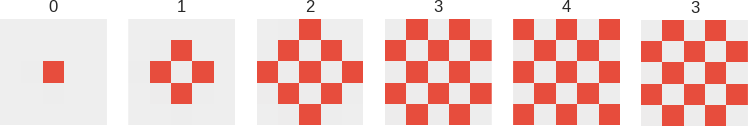
\includegraphics[height=0.4\textheight, width=\textwidth, keepaspectratio]{fig/result_figs/generate_mosaic/1}
\caption[Example CA]{An example binary 2D CA. At time step 5 the CA state is the same as that in time step 3, meaning the CA has entered a cyclical attractor with a period of 2 (oscillation).}
\label{fig:example_CA}
\end{figure}

%There are many properties of CA and of cellular computing that can be varied to produce different results \cite{sipper-1999}.
%In this paper we will define some further properties of CA as:
%\begin{itemize}
%    \item Structured as a 1D or 2D cartesian grid of cells.
%    \item Having uniform cells, sharing the same transition rules.
%    \item Having a finite discrete set of states that cells can have.
%    \item Synchronously changing states for all cells.
%\end{itemize}

%Examples that fit into this narrower definition include Von Neumann's cellular automaton \cite{von-neumann-1966}, Wolfram's elementary cellular automata (TODO cite) and Conway's Game of Life (TODO cite Conway).

%Figure \ref{fig:110} illustrates "elementarty CA 110", which has this property.
%This is an 1D CA, with successive states transitioning from the top to the bottom over time.
%Two different patterns stand out from the background.
%Over time they move towards each other and interact.
%This interaction is used in Cook's proof that CA 110 is Turing complete.
%
%\begin{figure}
%\centering
%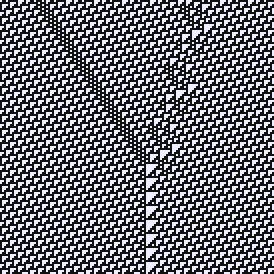
\includegraphics[width=\columnwidth]{fig/110}
%\caption{Elementary CA 110
%(TODO cite \protect\url{https://commons.wikimedia.org/wiki/File:Ca110-interaction.png} properly)}
%\label{fig:110}
%\end{figure}

%Since the inception of CA by Ulam and Von Neumann in the 1940s \cite{von-neumann-1966},
%researchers have been interested in them for their biology-like properties and emergent behavior.
%Most implementations of CA have been formal mathematical works or simulations on conventional computers,
%but work has also been done with physical implementations using various substrates (TODO cite).
%
%In recent times the problem posed by the end of Moore's law and he difficulty of parallel computing with conventional architectures has caused cellular computing to become relevant again.
%Michael J. Flynn created Flynn's Taxonomy in 1966 \cite{flynn-1966}, describing different types of parallel systems.
%In 1996 he wrote a new article \cite{flynn-1996},
%outlining some of the difficulties that had hindered the expected parallel processing power that he and his peers had imagined back then.
%In this article he also described what he thought to be the road ahead, which is to represent problems in cellular form.

\subsection{Transition Rules}
\label{sec:transitions}
Langton \cite{langton-1990} formally defined finite CA as consisting of a finite set of cell states $\Sigma$ of size $K = |\Sigma|$,
a finite input alphabet $\alpha$, and a transition function $\Delta$.
Each cell has a $N$-sized neighborhood.
The number of possible neighborhood states can be expressed by equation \eqref{eq:kn}.

\begin{equation}\label{eq:kn}
    |\alpha| = |\Delta| = |\Sigma^N| = K^N
\end{equation}

The transition function for a CA must thus encode $|\alpha|$ different mappings of $N$ inputs to one of $K$ outputs.
The number of possible unique transition function behaviors is thus $K^{(K^N)}$.

\begin{figure}
\centering
\begin{subfigure}[t]{.175\columnwidth}
\centering
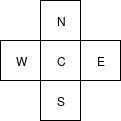
\includegraphics[width=\columnwidth]{fig/VonNeumann}
\caption{$N=5$ (Von Neumann)}
\label{fig:neighborhoods_vn}
\end{subfigure}\hfill%
\begin{subfigure}[t]{.175\columnwidth}
\centering
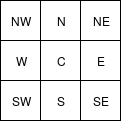
\includegraphics[width=\columnwidth]{fig/Moore}
\caption{$N=9$ (Moore)}
\end{subfigure}\hfill%
\begin{subfigure}[t]{.175\columnwidth}
\centering
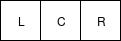
\includegraphics[width=\columnwidth]{fig/LCR}
\caption{$N=3$}
\end{subfigure}\hfill%
\begin{subfigure}[t]{.40\columnwidth}
\centering
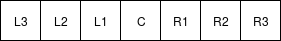
\includegraphics[width=\columnwidth]{fig/LLLCRRR}
\caption{$N=7$}
\end{subfigure}\hfill%

\caption[Some CA neighborhoods]{Some examples of common neighborhood shapes. The two common 2D shapes are named for John von Neumann and Edward F. Moore.
}
\label{fig:neighborhoods}
\end{figure}

\subsection{The $\lambda$ Parameter and the Edge of Chaos}
When Christopher Langton studied the elementary CA ($N=3, K=2$) \cite{langton-1990},
he created a metric to help determine if a rule is ordered, chaotic, or something in between, which he called $\lambda$.
It is defined by $K$, $N$ and the number of transitions that goes to the quiescent state, $n$.
\begin{equation}\label{eq:lambda}
    \lambda = \frac{K^N - n}{K^N}
\end{equation}

Langton found that low elementary CA $\lambda$ values resulted in ordered behavior, either settling into a static state or repeating periodically.
With high $\lambda$ values, the CA became chaotic, losing all useful information in the noise.
But at the critical border region between order and chaos, interesting behaviors and computation could occur \cite{langton-1990}.
This area has come to be called the \textit{edge of chaos}.

In the study Langton investigated the $\lambda$ of 1D binary CA, but the measure can be used on any CA.
The 2D binary transition function shown in Table \ref{tbl:example_CA} has 17 input combinations that lead to the quiescent ($0$) state ($n = 17$), and thus $\lambda \approx 0.47$.

\subsection{Finding Interesting Transition Functions}
\label{sec:finding_transitions}
\begin{table}
    \centering
    \caption[Example table-based transition rule]{
        An example table-based transition rule that exhibits the same behavior as seen in Figure \ref{fig:example_CA}.
        $N=5, K=2$ gives $|\alpha|=32$, the height of the table.
        The neighborhood shape is "Von Neumann" (Figure \ref{fig:neighborhoods_vn}).}
    \begin{tabular}{ccccc|c}
    North ($t_0$) & West ($t_0$) & Center ($t_0$) & East ($t_0$) & South ($t_0$) & Center ($t_1$) \\ \hline
    0      & 0      & 0      & 0      & 0      & 0        \\
    0      & 0      & 0      & 0      & 1      & 1        \\
    0      & 0      & 0      & 1      & 0      & 1        \\
    0      & 0      & 0      & 1      & 1      & 1        \\
    0      & 0      & 1      & 0      & 0      & 0        \\
    0      & 0      & 1      & 0      & 1      & 0        \\
    0      & 0      & 1      & 1      & 0      & 0        \\
    0      & 0      & 1      & 1      & 1      & 0        \\
    0      & 1      & 0      & 0      & 0      & 1        \\
    0      & 1      & 0      & 0      & 1      & 1        \\
    0      & 1      & 0      & 1      & 0      & 1        \\
    0      & 1      & 0      & 1      & 1      & 1        \\
    0      & 1      & 1      & 0      & 0      & 0        \\
    0      & 1      & 1      & 0      & 1      & 0        \\
    0      & 1      & 1      & 1      & 0      & 0        \\
    0      & 1      & 1      & 1      & 1      & 0        \\
    1      & 0      & 0      & 0      & 0      & 1        \\
    1      & 0      & 0      & 0      & 1      & 1        \\
    1      & 0      & 0      & 1      & 0      & 1        \\
    1      & 0      & 0      & 1      & 1      & 1        \\
    1      & 0      & 1      & 0      & 0      & 0        \\
    1      & 0      & 1      & 0      & 1      & 0        \\
    1      & 0      & 1      & 1      & 0      & 0        \\
    1      & 0      & 1      & 1      & 1      & 0        \\
    1      & 1      & 0      & 0      & 0      & 1        \\
    1      & 1      & 0      & 0      & 1      & 1        \\
    1      & 1      & 0      & 1      & 0      & 1        \\
    1      & 1      & 0      & 1      & 1      & 1        \\
    1      & 1      & 1      & 0      & 0      & 0        \\
    1      & 1      & 1      & 0      & 1      & 0        \\
    1      & 1      & 1      & 1      & 0      & 0        \\
    1      & 1      & 1      & 1      & 1      & 0        \\
    \end{tabular}
    \label{tbl:example_CA}
\end{table}

Traditionally $\Delta$ has been encoded as a complete mapping $\Delta: \Sigma^N \rightarrow \Sigma$, which can be implemented as a lookup table.
Table \ref{tbl:example_CA} shows an example of a table encoding for the CA in Figure \ref{fig:example_CA}.
This works very well for smaller cases such as the elementary CA.
But when working with non-trivial CA where both $K$ and $N$ can be relatively large numbers,
it becomes a problem both to store the mapping $\Delta$ in an efficient way,
and the space of possible $\Delta$ becomes too large to be explored by exhaustive enumeration.

Designing $\Delta$ with interesting behavior by hand is possible,
but it is time-consuming and impractical for problems of greater dimensions.
Using adaptive algorithms to explore the space of possible solutions is more feasible.
This is not guaranteed to produce good results though.
The use of table-based encodings put certain limitations on the search.
Using other encodings may enable new, more powerful search algorithms.
%This thesis concerns the investigation of a novel transition function encoding and associated search algorithm.

%\subsection{CA Problems}
%There are many kinds of problems that can be solved with CA.
%One class of problems is called \textit{morphology problems}.
%In these problems, the goal is for the CA to create some kind of complex structure.
%This can for example be \textit{morphogenesis}, where a simple structure is over time transformed into a more complex one,
%or it can be \textit{replication}, where some complex structure present initially must be copied.
%
%Another class of problems can be called \textit{information problems} (TODO is there a more appropriate term?).
%In this kind of problem the goal can be to compute some result based on the initial state, or to transmit information about state from one end to another.
%
%TODO citations
